\begin{section}{Results}
  \label{sec:results}
  We now present the results of a simulation of (**) neutrinos with mass 0.2eV and (**) dark matter particles. The simulation is done in a box of size $250 Mpc/h$. As noted above, initial conditions for dark matter particles are produced at $z=100$ whereas neutrinos are introduced at $z=10$. We take cosmological parameters which are in line with the most recent Planck results \cite{bib:Planck2015}: $h=0.67,\, \Omega_b=0.05, \Omega_c=0.27, \sigma_8=??,\, n_s=0.67 $, and

\begin{equation}
  \Omega_\nu = \frac{m_\nu}{93.14 h^2}
\end{equation}
We assume a flat universe and so set $\Omega_\Lambda=1-\Omega_m=1-\Omega_b-\Omega_c-\Omega_\nu$.
  TODO: Add results

\begin{figure}[htbp]
  \begin{center}
    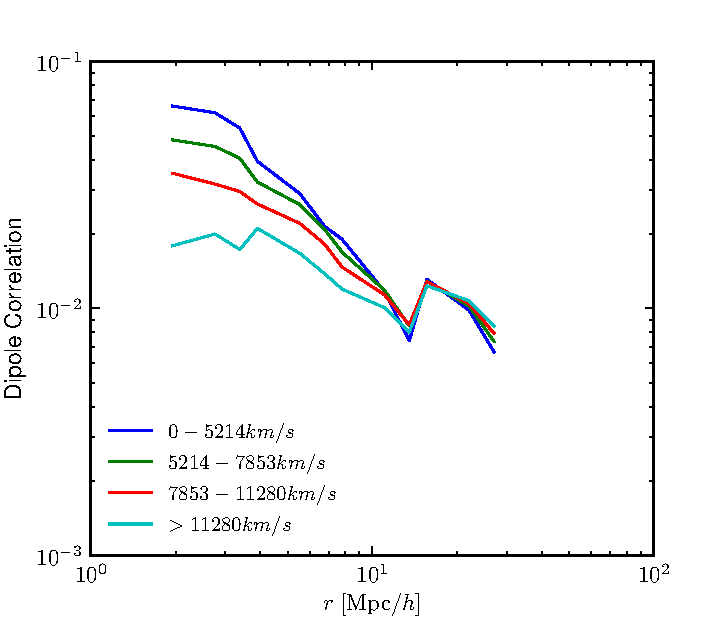
\includegraphics[width=0.5\textwidth]{./figures/Dipole/dipolefig.pdf}
    \caption{Dipole Placeholder}
    \label{fig:dipolefig}
  \end{center}
\end{figure}

\begin{figure}[htbp]
  \begin{center}
    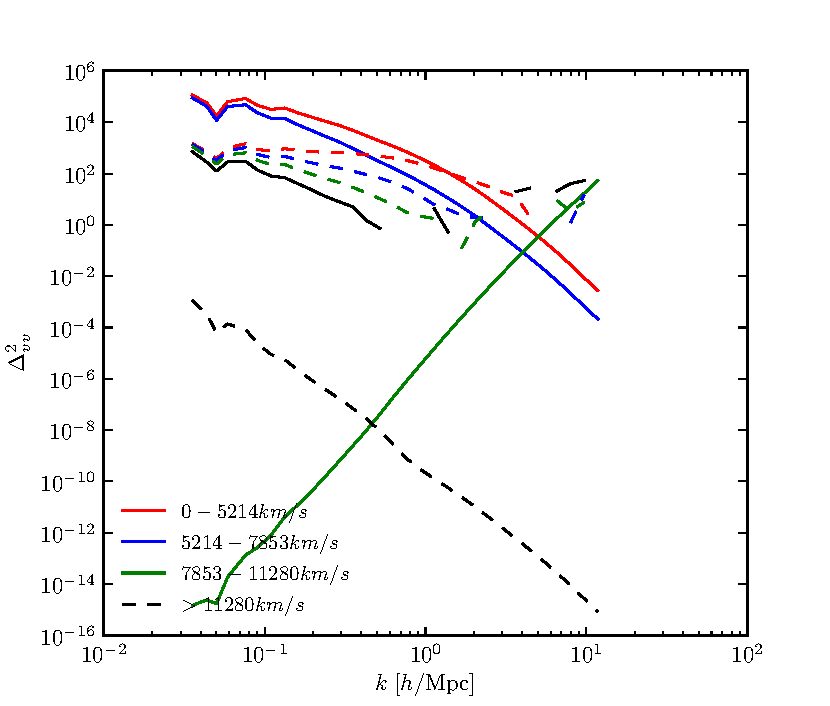
\includegraphics[width=0.5\textwidth]{./figures/VelPowerSpectra/velpower.pdf}
    \caption{Velocity Power Placeholder}
    \label{fig:velpowerfig}
  \end{center}
\end{figure}

\end{section}
